\newpage
\appendix
\chapter{Анализ мод в щели}
Уравнения на собственные значения $q_\nu$ получаются из условий непрерывности электрического и магнитного полей на стенках щели $x = \pm \ell$ и имеют вид для чётных мод:
\begin{equation}
    \begin{cases}
        \cos(q_\nu \ell) = T \\
        q_\nu \sin (q_\nu \ell)  = \frac{T}{\eps_M} q_{M_\nu},
    \end{cases}
    \label{eq:roots_even_ap}
\end{equation}
и для нечётных мод
\begin{equation}
    \begin{cases}
        \sin(q_\nu \ell) = T \\
        -q_\nu \cos (q_\nu \ell)  = \frac{T}{\eps_M} q_{M_\nu}. 
    \end{cases}
    \label{eq:roots_odd_ap}
\end{equation}

Деля одно уравнение на другое в каждой системе уравнений, получаются следующие трансцендентные уравнения
\begin{equation}
    \begin{cases}
        \eps\ \text{tg}(x_\nu) = \frac{\sqrt{(1-\eps)x_0^2  - x_\nu^2}}{x_\nu}, & \nu = 0,\ \pm 2,\ \pm 4, ... \\
        -\eps\ \text{ctg}(x_\nu) \frac{\sqrt{(1-\eps)x_0^2 - x_\nu^2}}{x_\nu}, & \nu = 1,\ \pm 3,\ \pm 5, ... \\
    \end{cases},
\end{equation}
где для краткости использованы обозначения $x_\nu = q_\nu \ell$ и $x_0 = k_0 \ell$. Выражая тригонометрические функции через экспоненты
\begin{equation*}
     \text{tg}(x) = \frac{e^{i x} - e^{-i x}}{i (e^{i x} + e^{-i x})}
\end{equation*}
и вынося $e^{-ix}$ как общий множитель, представленные выше трансцендентные уравнения переписываются в виде, представленном в главе 1
\begin{align}
e^{2i q_\nu l} &= \pm \frac{i-g(q_\nu,\varepsilon)}{i+g(q_\nu,\varepsilon)},\label{eq:BoundCond_ap} \\
g(q_\nu,\varepsilon) & = \frac{\sqrt{(1-\varepsilon)(k_0 \ell)^2 - (q_\nu l)^2}}{\varepsilon q_\nu l}.  \nonumber
\end{align}
Анализ корней этого уравнения для $\abs{\eps'}\gg 1$ и $\eps'' = 0$ представлен в главе 1. При расчётах амплитуд полей и силы используется метод Ньютона. 

Как уже было замечено, при $\eps \to -\infty$ корни уравнения стремятся к $\pi \nu/2\ell$. Тогда матричные элементы в системе уравнений ~(\ref{eq:General_System_ap})
\begin{align}
	\sum_{\nu=-\infty}^{+\infty} F_{\mu \nu} h_\nu = (1+R)f_{\mu,-k_{0x}} + \frac{(1-R)k_{0z} l}{\pi}\int f_{\mu,-k}\sinc((k_{0x}-k)l) \frac{dk}{\varkappa}, \label{eq:General_System_ap}
\end{align}
где 
\begin{align}
F_{\mu \nu} &= f_{\mu,\nu} + \frac{\beta_\nu}{2\pi}\int
\Bigl(f_{\nu,k}f_{\mu,-k}  + \frac{b_\nu(\ell)}{\eps} G(q_{M\nu},k)f_{\mu,-k} \Bigr)\frac{dk}{\varkappa}
\label{eq:F_mn_ap}
\end{align}
упрощаются. Для чётных гармоник 
\begin{align}
    f_{\mu,\nu} = \text{sinc}(q_\nu - q_\mu)\ell + \text{sinc}(q_\nu +q_\mu)\ell &\to \\
    \text{sinc}(\nu - \mu)\pi/2 + \text{sinc}(\nu +\mu)\pi/2& = \delta_{\nu,\mu}(1 + \delta_{\nu,0}). \nonumber
\end{align}
Для нечётных мод $f_{\mu,\nu}$ равен нулю. Второй интегральный член, содержащий $G(q_\mu,k)$ стремится к нулю при $\eps \to -\infty$. В правой части системы уравнений второй член стремится к нулю, так как 
$$
R = \frac{\eps \cos(\gamma) - \sqrt{\eps - \sin^2(\gamma)}}{\eps \cos(\gamma) + \sqrt{\eps - \sin^2(\gamma)}}\to 1.
$$
Перейдём от суммы по $\sum_{\nu = -\infty}^{+\infty}$ к сумме $\sum_{\nu = 0}^{+\infty}$ пользуясь тем фактом, что корни симметричны $q_\nu = -q_{-\nu}$. Тогда система приобретает вид
\begin{equation}
    h_\mu + \sum_{\nu = 0}^{+\infty}T_{\mu,\nu}h_\mu = f_{\mu,-k_{0_x}}
\end{equation}
где новые матричные элементы 
\begin{equation}
    T_{\mu,\nu} = \frac{\ell}{4 \pi}\beta_\mu (2 - \delta_{\mu,0})\int
\frac{f_{\nu,k}f_{\mu,-k}}{\varkappa}dk.
\end{equation}
При нормальном падении правая часть равняется $2 \delta_{\mu,0}$. Полученная система совпадает с результатами работ~\cite{Shapiro16,sturman2010transmission}.
\chapter{Моделирование бесконечности в численных методах}
Так как в задачах рассеяния часто встречается необходимость найти только рассеянное поле, а в методе конечных элементов расчётная область всегда ограничена, то было разработано несколько методов, моделирующих открытые границы. Для этого существует два подхода: использование специализированных граничных условий, либо изменение самого уравнения вблизи границы, которое обеспечивает безотражательное поглощение волны в этой области.

В случае, когда рассматриваются периодические структуры, то естественным образом является использование периодических граничных условий. В этом случае происходит даже упрощение задачи с точки зрения вычислительных мощностей, уменьшается количество независимых переменных. В ином случае используется численное приближение условия излучения Зоммерфельда~\cite{bayliss1982boundary}
\begin{equation}
    \frac{\partial u}{\partial r}+i k u = o(\frac{1}{r}), \ r\to \infty.
    \label{eq:Zommerfeld}
\end{equation}
Первая грубая аппроксимация этого условия даёт граничное условие излучения первого порядка (First order boudndary condition, 1st SBC)
\begin{equation}
    \textbf{n}\cdot \nabla u+i k u = 0.
    \label{eq:SBC_1}
\end{equation}
Оно действительно гарантирует полное прохождение падающей волны без отражения лишь при нормальном падении волны на границу, при росте угла падения, коэффициент отражения увеличивается. Этот тип условий реализован в COMSOL, однако разработчики не рекомендуют его использовать в силу его низкой точности. Фактически, имеется возможность получить аппроксимацию условия~(\ref{eq:Zommerfeld}) любого порядка по $1/r$ (см. работу~\cite{bayliss1982boundary}). В COMSOL реализовано условие излучение второго порядка (Second order boundary condition, 2nd SBC), которое имеет вид
\begin{equation}
    \textbf{n}\cdot \nabla u+i k u - \frac{i}{2 k} \nabla^2_\tau u= 0.
    \label{eq:SBC_2}
\end{equation}
Член $\nabla_\tau$ соответствует градиенту по касательной к границе, таким образом достигается повышение точности для волн, падающих под наклоном. Однако в COMSOL реализован первый тип условий по умолчанию, но разработчики рекомендуют использовать условие второго рода.

Ещё один способ смоделировать бесконечность --- это изменить уравнение вблизи границы. Такой подход называется идеально согласованными слоями (Pefectly Matched Layers, PML), и идейно состоит в замене обычной производной~\cite{nataf2013absorbing}
\begin{equation}
    \partial_x \to \partial^{pml}_x =\frac{i \omega}{i \omega + c \sigma(x) }\partial_x.
\end{equation}
Введение коэффициента $\sigma$ приводит к тому, что решение уравнения Гельгольца в PML зоне будет иметь вид
\begin{equation}
    u(x) =\alpha e^{(1+\frac{c \sigma}{i \omega})\frac{i \omega}{c}\sqrt{1-\frac{c^2 k^2}{\omega^2}}}+ \beta e^{-(1+\frac{c \sigma}{i \omega})\frac{i \omega}{c}\sqrt{1-\frac{c^2 k^2}{\omega^2}}},
\end{equation}
а коэффициент отражения от границы $R = \abs{\alpha/\beta}$ будет равен
\begin{equation}
    R = e^{-2\sqrt{1-\frac{c^2 k^2}{\omega^2}}\sigma \delta} = (e^{-2\sigma \delta})^{\cos(\theta)},
\end{equation}
где $\delta$ ширина PML области, $\theta$ угол между нормалью к поверхности PML слоя и подающей волны. Из этой формулы следует, что если взять достаточно большую ширину слоя, то отражение всегда будет равно нулю, кроме углов $\theta \approx \pi/2$, однако дискретизация области всё же приводит к появлению некоторого ненулевого коэффициента отражения, который пропорционален $\sigma \Delta x$. Использование более мелкого разбиения приводит к уменьшению отражения, а так же переменного $\sigma(x) = C x^2/\delta$. На практике $C \approx 20-40$, а $\delta \approx \lambda$. Таким образом, PML намного проще в использовании, по сравнению с граничными условиями первого рода, но требует больших вычислительных мощностей за счёт увеличения расчётной области. Сравнение коэффициентов отражения для условий излучения первого и второго порядка, а также PML слоя, представлены на~\ref{fig:PML_angle_dep}. График демонстрирует, что наименьший коэффициент отражения для всех типов условий достигается при углах, близких к нормали (поэтому цилиндрическая геометрия лучше подходит для цилиндрически рассеянных волн), но  наилучшим подходом всё-таки являются PML слои.
\begin{figure}
    \centering
    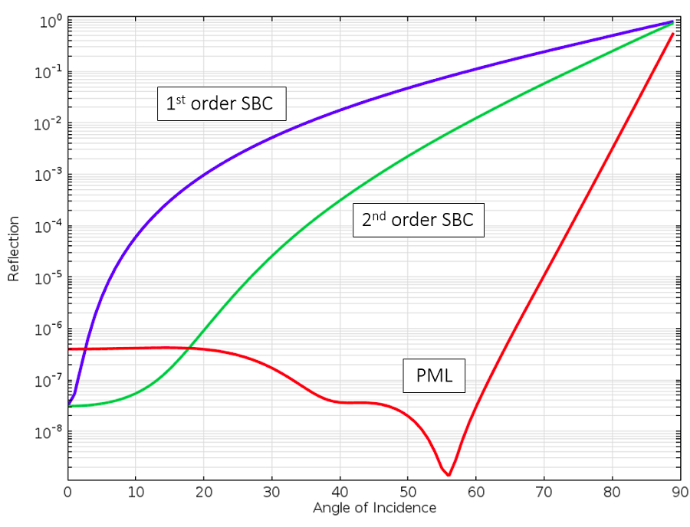
\includegraphics[width = \textwidth]{figures/PML_refl.png}
    \caption{Зависимость коэффициента отражения от PML слоёв от угла падения~\cite{Refl_PML}.}
    \label{fig:PML_angle_dep}
\end{figure}
\chapter{Предварительные данные эксперимента}
Установка для прецизионного измерения сил представлена на Рис.~\ref{fig:exp_set_up}. Излучение заводится между пластинами 6 и 7, которые представляют собой слой золота толщиной 200 мкм на керамической подложке. Изначально пластины представляли собой единый кристалл, но после были разделены на две, чтобы добиться большей гладкости. Золото после наращивалось отдельно, и из-за особенностей роста на поверхности золота образовались неровности, которые достигают высоты до $2$ мкм. Это одна из причин, по которой не удаётся произвести измерения для субволновой щели.

Излучение заводится с помощью оптического волокна с сохранением поляризации. Изменение поляризации производится непосредственным вращением волокна. Система позиционирования позволяет выполнить шестикоординатную юстировку падающего излучения и пластин. Контроль положения пластины-датчика обеспечивается за счёт системы из кремниевого маятника и электродов. Параллельное смещение маятника измеряется с помощью интерферометра, а повороты вокруг вертикальной и горизонтальной осей при помощи квадрантного фотодетектора.
\begin{figure}
    \centering
    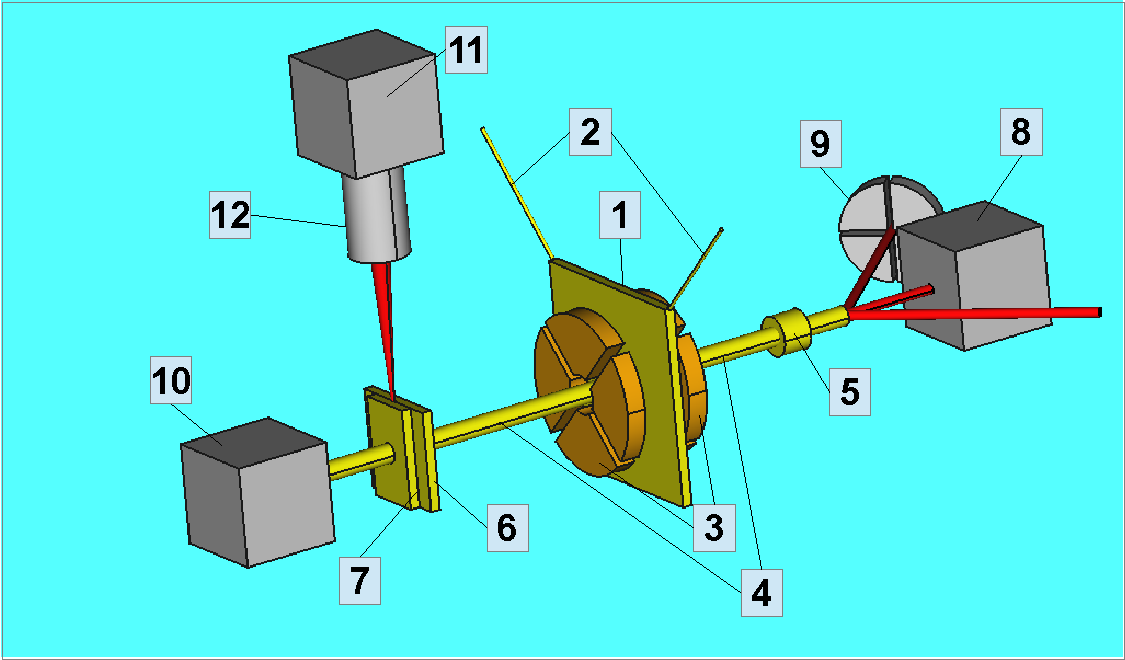
\includegraphics[width=\textwidth]{figures/exp2.pdf}
    \caption{Схема экспериментальной установки: 1 --- маятник, 2 --- подвес, 3 --- электроды,  4 --- керамический стержень, 5 --- противовес, 6 --- пластина-датчик, 7 --- пластина-образец, 8 --- интерферометр, 9 --- квадрантный фотодетектор, 10 --- система позиционирования образца, 11 --- система позиционирования оптического волокна, 12 --- вращатель волокна.}
    \label{fig:exp_set_up}
\end{figure}

Помимо неровности пластин, в эксперименте сказываются другие эффекты, которые усложняют процесс измерения. Один из таких эффектов --- это тепловое расширение. На установке используется специальный керамический стержень с малым коэффициентом теплового расширения для соединения датчика силы с маятником. Однако пластины сами нагреваются в течении эксперимента, из-за чего тоже деформируются, что трудно учесть. Так же неопределённость в значение силы вносят электростатические заряды, случайно распределённые на поверхности пластин. Для компенсации этого эффекта был разработан специальный метод подачи периодически меняющегося напряжения на пластины.

В ходе эксперимента было проведено измерение светоиндуцированной силы, и предсказанный эффект притяжения был зарегистрирован. Однако имеются значительные количественные расхождения между экспериментом и теоретическими расчётами. На Рис.~\ref{fig:force_exp} представлена зависимость измеренной силы в эксперименте, а на Рис.~\ref{fig:force_N_2eps_1} и~\ref{fig:force_N_2eps_2} представлен теоретический расчёт силы при заданной мощности при различных значениях проницаемости. Видно что в эксперименте не наблюдается монотонного спада силы при малых расстояниях. Это может быть связано с неровностями пластин. После положения пластины $1$ мкм в эксперименте и в расчёте наблюдается плато, на котором величина силы практически не меняется. Однако, если сравнить расчётное значение силы при литературном значении $\eps = -100+10i$ с экспериментом, то количественное расхождение составляет примерно $200$ раз.  Между значениями $1.5$ и $2$ мкм расчётная величина остаётся неизменной, в то время как измеренная плавно спадает до нуля. Далее сила меняет знак и становится отталкивающей. Этот эффект можно объяснить рождением второй чётной моды (в ходе эксперимента была определена контактная точка пластин при положении пластины-образца $0.5$ мкм, а значит порог рождения первой чётной моды при ширине щели $1.5$ мкм соответствует положению платины $2$ мкм). Здесь наблюдается качественное расхождение с теорией, так как  значение проницаемости $-100 + 10i$ не воспроизводит эффект отталкивания. Однако, как было показано в главе 2, этот эффект возможен при других значениях проницаемости, например $\eps = -360+60i$, но в этом случае большее значение мнимой части $\eps$ приводит к ещё меньшему значению силу. 

В связи с тем, что варьирование значений $\eps'$ и $\eps''$ даёт возможность приближённо воспроизвести экспериментальную кривую (см. Рис.~\ref{fig:force_N_2eps_2}), нами была выдвинута гипотеза о том, что литературное значение проницаемости золота не соответствует реальному. В действительности, мы использовали значение проницаемости бесконечного кристалла, а в эксперименте вклад основной вклад играют электроны на поверхности. В работе~\cite{laref2013size} авторы изучили вклад толщины золота в значение проницаемости, используя Density Function Theory (DFT) подход. Авторы смоделировали плёнки из золота в вакууме толщиной $1-7$ нм и рассчитали значения проницаемости. Результат моделирования выявил сильную анизотропию и большой вклад толщины плёнок в величину проницаемости. Однако полученные авторами значения $\eps''$ не опускаются ниже единицы, в связи с этим сложно утверждать, что выбранные нами тестовые значения $\eps$ физически реализуемы ($\eps'' = 0.2,\ 0.04$). Но стоит отметить, что в рассмотренной работе эффекты, связанные с возникновением ненулевой $\eps''$, такие как электрон-электронное рассеяние, электрон-фононное и рассеяние электронов на примесях, не рассчитываются и входят как внешний параметр, измеренный экспериментально для бесконечного кристалла~\cite{blaber2009search}.

В действительности, есть возможность оценить реальное значение мнимой части проницаемости в настоящем эксперименте. Для измерений используются пластины длиной $40$ мм, и для значения проницаемости $\eps = -100 + 10i$ максимальная характерная глубина проникновения (при ширине щели  $2.5$ мкм),  достигает 2 мм, а значит, если установить фотодетектор за щелью, на выходе сигнала быть не должно. Если же взять значения $\eps = -300 + 0.2i$ или $\eps = -100+0.04$, то характерная глубина проникновения достигает $40$ см. Таким образом, измеряя сигнал с фотодетектора, можно оценить $\eps''$. Однако следует отметить, что в этом случае представленная нами теория уже неприменима, так как нужно учитывать отражение от выхода из щели. В связи с этим, требуется расширении теории.

\begin{figure}
    \centering
    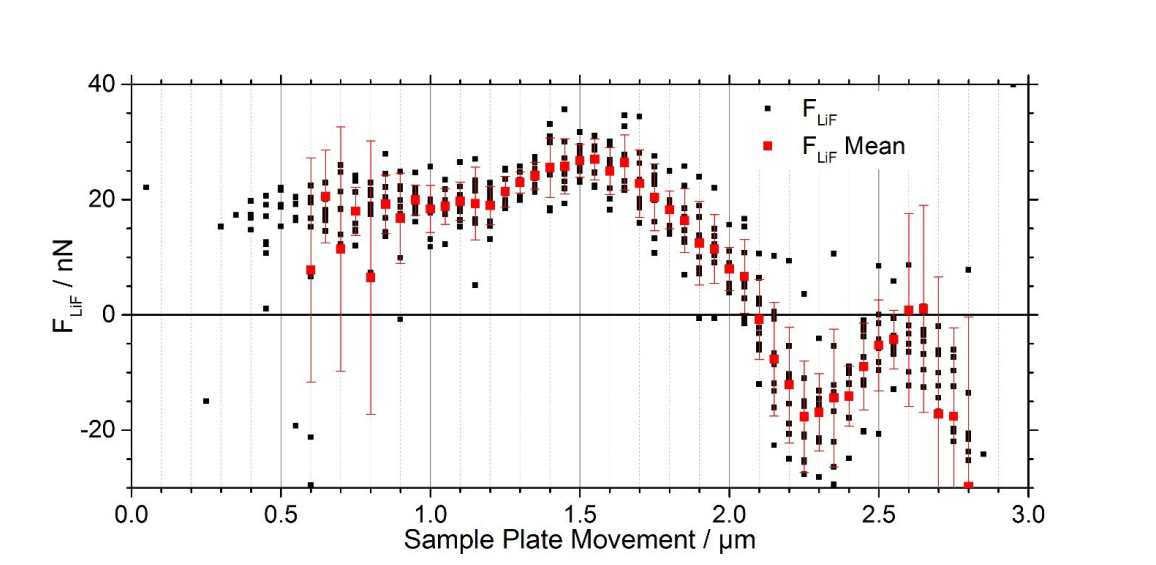
\includegraphics[width=\textwidth]{figures/exp_data_force.png}
    \caption{Измеренная сила в зависимости от положения пластины-образца. Точка контакта пластин соответствует положению $0.5$ мкм.}
    \label{fig:force_exp}
\end{figure}
\begin{figure}
    \centering
    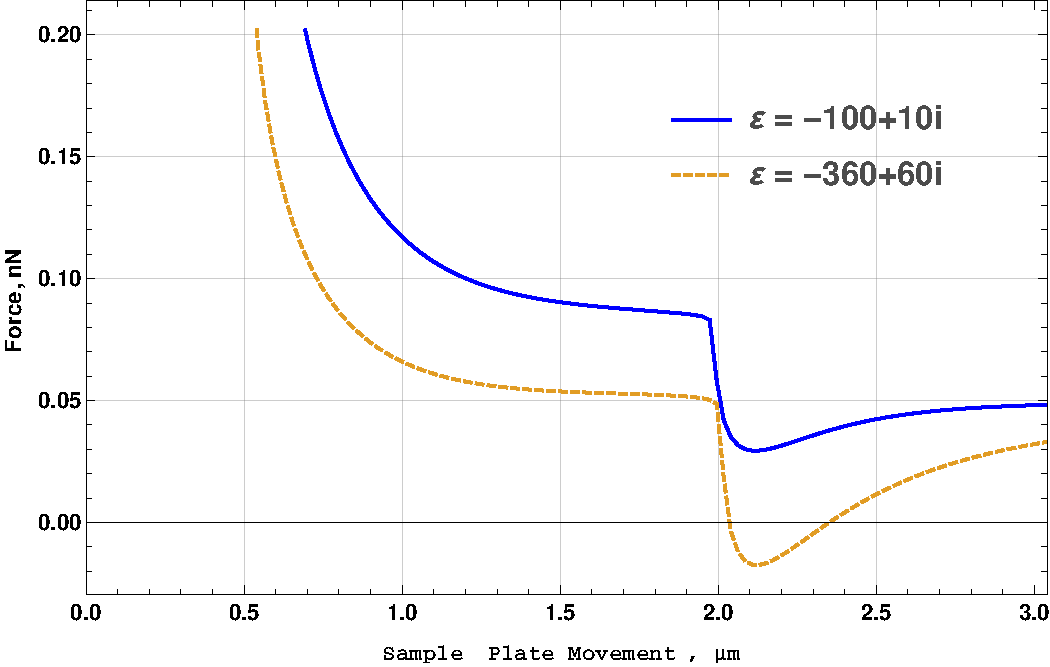
\includegraphics[width=\textwidth]{figures/ForceGauss_Newton_10010_36060.pdf}
    \caption{Рассчитанная сила в зависимости от ширины щели при $\eps = -100 + 10i$ (сплошная линия) и $\eps = -360+60i$ (пунктирная линия).}
    \label{fig:force_N_2eps_1}
\end{figure}
\begin{figure}
    \centering
    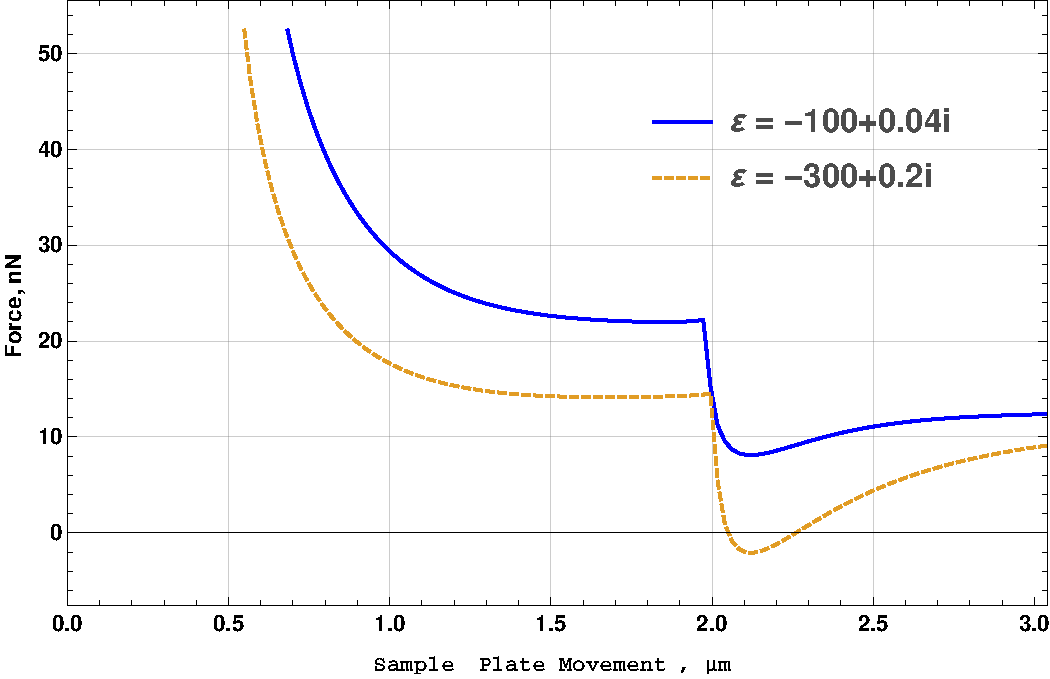
\includegraphics[width=\textwidth]{figures/ForceGauss_Newton_100_004_300_02.pdf}
    \caption{Рассчитанная сила в зависимости от ширины щели при  $\eps=-100+0.02i$ (сплошная линия) и $\eps = -300 + 0.1i$ (пунктирная линия).}
    \label{fig:force_N_2eps_2}
\end{figure}


